% -*- fill-column: 85; -*-
%!TEX root = ../dissertation.tex

\section{Evaluation}
\label{s:eval}

\AvA was evaluated on an Intel Xeon E5-2643 CPU with 128~GiB DDR4 RAM, using
Ubuntu~18.04 LTS, and Linux 4.14 with modified KVM and vhost modules. Guest
VMs were assigned 4 virtual cores, 4~GiB memory, 30~GB disk space, and ran
Ubuntu~18.04 LTS with the stock Linux 4.15 kernel. \workers and VMs were
co-located on the same server for all experiments except live migration and
the FPGA benchmarks. Experiments involving a Google Cloud TPU were carried out
on a Google Compute Engine instance with 8 vCPUs (SkyLake), 10~GiB memory, and
a disaggregated Cloud TPU v2-8 in the same data center. The guest VM was
located on the same instance via nested virtualization. Experiments for the
custom FPGA API were done on an AWS F1 \lstinline|f1.2xlarge| instance (with 1
Virtex UltraScale+ FPGA, 8 vCPUs, and 122 GiB memory). For live migration, a
second similar server was used as the remote machine, and the servers were
directly connected by 10 Gigabit Ethernet.

\subsection{Development Effort}
\label{s:eval_effort}

\definecolor{Gray}{gray}{0.9}
\begin{table}
	\footnotesize
    \newcolumntype{\N}{S[table-format=4.0, table-alignment = right, table-auto-round = true]}
    \newcolumntype{\n}{S[table-format=1.0, table-alignment = right, table-auto-round = true]}
    \setlength{\tabcolsep}{3pt}
	\begin{tabular}{lcrrrll}
    \toprule
	API                         & Gen              & {\#}                 & {LoC}                  & {Churn}                 & Benchmark                & Hardware                                      \\
	\midrule
	\multirow{2}{*}{OpenCL~1.2} & \cross \cellcolor{Gray} & {\cellcolor{Gray}}39 & {\cellcolor{Gray}}7514 & {\cellcolor{Gray}}14318 & \multirow{2}{*}{Rodinia} & \multirow{2}{7em}{NVIDIA~GTX~1080 AMD~RX~580} \\
                                & \checkmark       & 38                   & 1060                   & 2868                    &                          &                                               \\
	CUDA 10 Driver              & \checkmark       & 16                   & 266                    & 410                     & Rodinia                  & NVIDIA~GTX~1080                               \\
	CUDA 10 Runtime             & \checkmark       & 93                   & 1358                   & 1973                    & Rodinia                  & NVIDIA~GTX~1080 								\\
	TensorFlow~1.12~C           & \checkmark       & 46                   & 501                    & 887                     & Inception                & NVIDIA~GTX~1080                               \\
	TensorFlow~1.13~Py          & \cross           & {\scriptsize n/a}    & 3245                   & 5972                    & VGG-net Inception        & Google~Cloud TPU v2-8                         \\
	TensorFlow~1.14~Py          & \checkmark       & 111                  & 1865                   & 2557                    & Neural networks          & NVIDIA~GTX~1080 								\\
	TensorFlow Lite~1.13        & \cross           & {\scriptsize n/a}    & 1295                   & 2005                    & Official examples        & Coral Edge~TPU                                \\
	NCSDK~v2                    & \checkmark       & 26                   & 479                    & 1279                    & Inception                & Movidius~NCS v1                         \\
	GTI SDK~4.4                 & \checkmark       & 38                   & 284                    & 568                     & Official examples    & Gyrfalcon 2803 Plai Plug                         \\
	Custom FPGA on AmorphOS~\cite{amorphos}     & \checkmark       & 4                    & 30                     & 40                      & BitCoin  & AWS~F1                                        \\
	QuickAssist~1.7             & \checkmark       & 19                   & 444                    & 676                     & QATzip                   & Intel~QAT 8970                      \\
	HIP                         & \checkmark       & 41                   & 624                    & 990                     & Galois~\cite{tao}        & AMD~Vega~64                                   \\
	\bottomrule
	\end{tabular}
	\caption{Development effort for forwarding different APIs, along with the benchmarks~\cite{inceptionv3,vggnet,rodinia} and hardware used to evaluate them. The \textbf{\#} column indicates the number of API functions supported. The Python APIs are forwarded dynamically, making \# inapplicable. \textbf{Gen} indicates whether the API forwarding was generated by \CAvA or was written by hand. \textbf{LoC} is the number of lines of code (including blank lines and comments) in the \CAvA specification or C/Python code. \textbf{Churn} is the total number of lines modified in commits.}
	\label{tab:apis-and-accs}
\end{table}

Table~\ref{tab:apis-and-accs} presents the \numframeworks APIs and
\numaccelerators devices virtualized using \hira (either by hand or with
\CAvA). Automation provided by \CAvA enables significant reduction in
developer effort when virtualizing APIs according to the \hira design. In
order to understand developer effort, we use the lines of \lapis specification
or C/Python code (\texttt{LoC} in Table~\ref{tab:apis-and-accs}), and the
number of lines of code modified (\textbf{Churn} in
Table~\ref{tab:apis-and-accs}) during development (counted from commits) as
indicative of effort. Larger \texttt{LoC} and \textbf{Churn} represents higher
effort expended to build the virtualization scheme for that API. Overall, we
find that the automation afforded by \lapis and \CAvA enable much APIs to be
virtualized at much lower effort and in much shorter time frames.
For example, our hand-rolled OpenCL API remoting system, which supports the
parts of the OpenCL API needed to run the Rodinia~\cite{rodinia} benchmarks,
took more than 3 developer-months to build, and the resulting artifact had
7,514 LoC (see row 1 of Table~\ref{tab:apis-and-accs}).
Supporting the same subset of OpenCL with \lapis and \CAvA, took a single
developer a little over a week, and the resulting API specification was 1,060
LoC long. Even in cases where we couldn't leverage \AvA---TensorFlow and
TensorFlow Lite Python APIs---leveraging \AvA's API-agnostic components
enabled us to build a \hira system with reasonable effort (3,245 lines of
Python code and 2 developer weeks for TensorFlow Python).

\begin{sidewaysfigure}
	\centering

	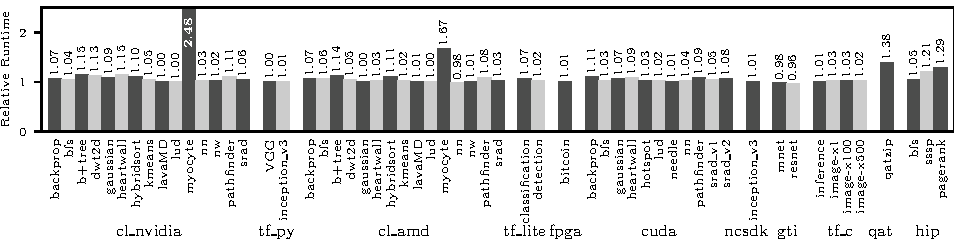
\includegraphics[width=\linewidth]{ava/data/end2end/end2end_all.pdf}
	\caption{End-to-end execution time on virtualized APIs or accelerators
	normalized to native execution time. \lstinline|tf_py| is the handwritten
	TensorFlow Python API remoting with \AvA API-agnostic components.}
	\label{fig:end2end}

	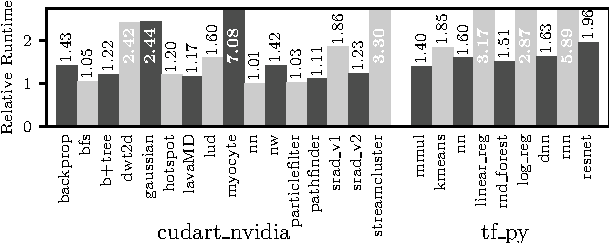
\includegraphics[width=0.6\linewidth]{ava/data/end2end/end2end_cudart.pdf}%
	\vspace*{-.1em}
	\caption{End-to-end execution time on virtualized CUDART and CUDA-accelerated TensorFlow APIs normalized to native execution time.}
	\label{fig:end2end_cudart}

\end{sidewaysfigure}

\subsection{End-to-end Performance}

Figure~\ref{fig:end2end}--\ref{fig:end2end_cudart} shows the end-to-end
runtime, normalized to native, for all benchmarks, accelerator and API
combinations we support (see Table~\ref{tab:apis-and-accs}).
\AvA introduces modest overhead for most workloads. Excluding the
\texttt{myocyte} benchmark, the Rodinia OpenCL benchmark suite on NVIDIA GTX
1080 GPU slowed down by 7\% on average. The outlier, \texttt{myocyte} has over
2$\times$ overhead because it is extremely \textbf{call-intensive}---it
makes over 200,000 calls in \SI{18.5}{\second}; most others make between 30
and 3,000 calls. \texttt{Myocyte} experienced lower overhead on the AMD Radeon
RX 580 GPU, as the kernels executed 3$\times$ slower, allowing more of \AvA's
overheads to be amortized. The benchmarks for CUDA runtime API and
CUDA-accelerated TensorFlow are mostly call-intensive. The geometric mean
overhead is 79.6\%, 4$\times$ faster than FlexDirect.

The TensorFlow benchmarks for the handwritten Python API remoting system, and
Movidius benchmarks show low overhead---0\% overhead on VGG-net running on
TensorFlow Python (Cloud TPU), and 7\% slowdown for image classification on
TensorFlow Lite (Coral Edge TPU)---as they are \textbf{compute-intensive}.
Each offloaded kernel performs a lot of computation per byte of data
transferred, with relatively few API calls. The Gyrfalcon benchmarks enjoy a
slight speedup as time spent loading and initializing the library are
eliminated by using a pre-spawned \worker pool. The QuickAssist accelerator
proved challenging to virtualize, as it is a high-data-rate kernel-bypass
encryption/compression accelerator. Applications that run on this device are
\textbf{data-intensive}: computation per transferred byte is very low. We ran
the Intel QATzip compression application on the Silesia corpus~\cite{silesia}
using synchronous QAT APIs: while the application only experienced a
1.38$\times$ end-to-end runtime slowdown, its throughput was 2.2$\times$ lower
on average. \AvA was not able to keep up with the high throughput of the
device, due to data transfer and marshalling overheads, as the time spent
transferring data between the guest and the host was equivalent to compute
time on the accelerator. Zero-copy between the VM and the host might
ameliorate this overhead. We note that QAT on \AvA is fair, unlike the onboard
SR-IOV support.

Overall, the end-to-end experiments show that, \ava, our realization of the
\hira virtualization design, introduces very low overheads for most workloads
and is competitive with user-space API-remoting. This confirms our hypothesis
that \hira represents a ``sweet-spot'' in the DSA virtualization design space.

\subsection{Micro-benchmarks}
\label{s:micro_benchmark}

\begin{figure}[!!!ht!]
	\centering
	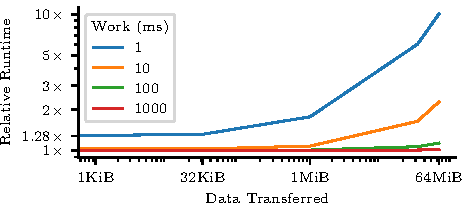
\includegraphics[width=0.7\linewidth]{ava/data/microbenchmark/overhead_plot.pdf}%
    \vspace*{-.5em}
	\caption{Overhead introduced by \AvA for a micro-benchmark with varying work per call and data per call. The plot is log-log and the trend is linear. Runtime is relative to running the same micro-benchmark natively on the NVIDIA GTX 1080 GPU.}
	\label{fig:microbenchmark_overhead}
\end{figure}

Given that our benchmark applications can be classified as being
compute-intensive, data-intensive, and call-intensive, it would be instructive
to understand the impact of the \hira design for each of these classes of
workloads. To that end, we crafted a micro-benchmark that mimicked each of
these classes of applications by varying the amounts of data transferred to
the GPU per call, and the duration of computation per call (simulated by
spinning on the host). Figure~\ref{fig:microbenchmark_overhead} shows that
\emph{compute-intensive} applications (represented by the lines for 100~ms and
1,000~ms of work) suffer the lowest overhead, as data transfer is amortized by
time computing on that data. \emph{Data-intensive} applications (represented
by the 1~ms and 10~ms lines) experience severe slowdowns as the data
transferred per call increases, such as when 64~MiB is moved for only 1~ms of
compute. \emph{Call-intensive} applications (represented by the 1~ms line on
the left side of the graph) transfer small amounts of data and execute
relatively short kernels, so control transfer dominates execution, (e.g. 28\%
overhead on 1~ms calls with no data).

\subsubsection{Asynchrony Optimizations}
\label{s:opt_eval}

\begin{figure}[!th]
	\centering
	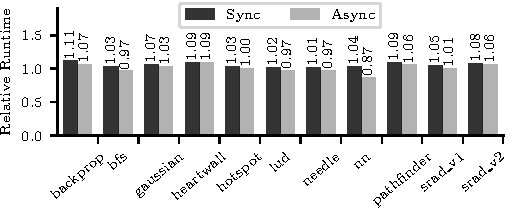
\includegraphics[width=0.7\linewidth]{ava/data/end2end/end2end_async.pdf}%
	\caption{End-to-end runtime of CUDA benchmarks (relative to native) using synchronous and asynchronous specifications.}
	\label{fig:eval_async}
\end{figure}

Synchronous APIs calls that have no output of any kind remain semantically
correct if executed asynchronously. For example, \lstinline|clSetKernelArg| is
a synchronous OpenCL API, but can be forwarded asynchronously to reduce the
overhead of these calls. The application's execution will not be faithful to
native execution, as the library would return immediately after the command is
sent to the \worker. Any resulting errors will be delivered from a later API
call. Similar techniques were applied in vCUDA (lazy RPC)~\cite{vCUDA} and
rCUDA (API batching)~\cite{rCUDA}.

In order to understand the effectiveness of this optimization, We annotated
several synchronous APIs---\lstinline[breaklines=true,escapechar=|]@cuLaunchKer@\-\lstinline@nel@, \lstinline@cuMemcpyHtoD@, and resource free functions---to
be asynchronous. Figure~\ref{fig:eval_async} shows that this optimization
results in a 5\% speedup on average (geometric mean) in end-to-end runtime (
normalized to native) for CUDA Rodinia benchmarks.

\subsection{Scalability}
\begin{figure}[!th]
	\centering
	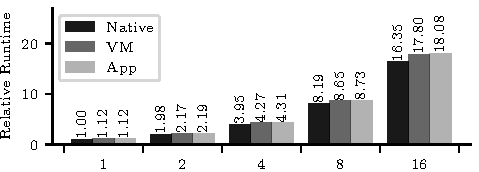
\includegraphics[width=.7\linewidth]{ava/data/scalability/scalability.pdf}%
	\caption{Scalability of \ava when supporting multiple VMs running a single application each (\textbf{VM} bars in figure), and multiple applications in a single VM (\textbf{App} bars in figure). Runtime is relative to running a single application natively (native scalability is shown with the \textbf{Native} bars.}
	\label{fig:scalability}
\end{figure}

To evaluate scalability, we ran multiple instances of the OpenCL
\texttt{gaussian} benchmark simultaneously in a number of different setups on a
NVIDIA GTX 1080 GPU: natively, all applications in one VM, and one VM per
application. A single instance of the \texttt{gaussian} benchmark fully
saturates the GPU. Overhead due to \AvA ($\sim$10\%) does not increase as the
number of VMs or applications increases, as shown by the near-perfect scaling
in Figure~\ref{fig:scalability}. The GPU kernel execution has an average 5.7\%
slowdown each time the number of VMs and applications is doubled. This
slowdown is small due better utilization of the physical device and other
system resources (e.g., when an instance of \textit{guassian} in one VM is
stalled, other instances can utilize the GPU.

Accelerators without process-level protection or sharing support (e.g., Intel
Movidius NCS) do not scale with \AvA (or any other virtualization scheme), as
multiple applications attempting to use the device have to be serialized.
\AvA added modest overheads (11\%) in a case where 4 VMs were all running
inception on the NCS v1. We note that \AvA still provides benefit by enabling
a hypervisor to expose and share the device across guest VMs.

\subsection{Guaranteeing fairness by Rate Limiting APIs}
\label{s:eval_rate_limit}

\begin{figure}[!!ht]
	\centering
    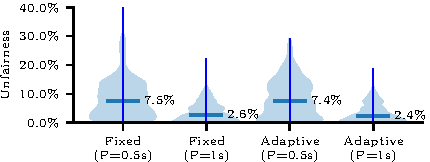
\includegraphics[width=0.7\linewidth]{ava/data/rate_limit/bias_plot.pdf}%
    \vspace{-.35em}
	\caption{Unfairness of the fixed and adaptive scheduling algorithms with two different measurement periods.The width of the shaded areas show the probability of the bias (unfairness) being a specific value in any given measurement window. The horizontal bar shows the median and the vertical line runs from the minimum to the maximum.}
	\label{fig:fairness}
\end{figure}

To evaluate whether \ava can guarantee fairness, we repeatedly executed
kernels drawn from six CUDA OpenCL benchmarks in pairs simultaneously in two
VMs on the NVIDIA GTX 1080 GPU. The kernels' execution time ranges from 1~ms
to 100~ms. Figure~\ref{fig:fairness} shows the fairness of the execution with
fixed-rate polling and feedback control method in 500-ms and 1-s measurement
windows. We compute unfairness as $\left|t_1-t_2\right| \mathbin{/} (t_1+t_2),$
where $t_i$ is the device time used by VM$_i$ in the time window.
For fixed-rate polling ($p=5$~ms), median unfairness in a \SI{1}{\second}
window is 2.6\%, and scheduling overhead was 7\%. For feedback control
($a=1$~ms and $b=1/2$), median unfairness is 2.4\% in a \SI{1}{\second}
measurement window, with 15\% overhead.


\subsection{Live Migration}

\begin{figure}[!ht]
	\centering
	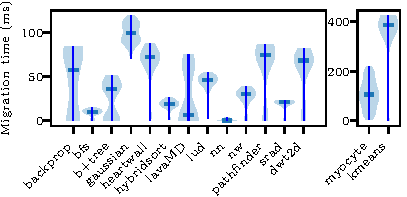
\includegraphics[width=0.7\linewidth]{ava/data/migration/time_plot.pdf}%
	\caption{Live migration downtime for single-threaded OpenCL benchmarks on NVIDIA GTX 1080. This downtime is in addition to the $\sim$\SI{75}{\milli\second} of downtime of the VM migration itself. Migration downtime does not include time spent waiting for executing kernels to complete (accounted as latency), as the application is still performing useful computation on the accelerator during that time. The width of the shaded areas show the the probability of a migration taking that length of time. The horizontal bar shows the median and the vertical line shows the range from minimum to maximum.}
	\label{fig:migration}
\end{figure}

\AvA's live-migration scheme uses annotations and selective record-and-replay instead of replaying the entire application on the remote.
To understand the efficacy of this scheme, we live-migrated a VM with 4~GB
memory, that was running OpenCL applications from the Rodinia benchmark suite,
between two servers that were directly connected via a 10~Gib Ethernet link,
both equipped with NVIDIA GTX 1080 GPUs. Migration was triggered at random
points in each benchmark, and the application could not make API calls for the
duration of the migration. Migrating the VM without \AvA or GPU usage takes
\SI{19}{\second} with a \SI{75}{\milli\second} downtime on average.
Figure~\ref{fig:migration} shows the downtime experienced by applications in
the VM, not including downtime for migrating the VM itself. 200 samples were
collected for \texttt{myocyte}, 150 for \texttt{gaussian} and \texttt{lud},
and 50 for all others.

The dominant cost is command transfer and replay, but this cost is also
affected by the size of the benchmark's state. Figure~\ref{fig:migration}
shows a bimodal distribution of downtime for most benchmarks. This is an
artifact of applications allocating device memory before entering a steady
execution state, and freeing it at termination. Migrations that occur before
device memory allocation do not need to transfer significant state; migrations
that occur after device memory allocation do.